En aquesta secció es descriuen les tècniques de visió per ordinador i tractament d'imatges emprades durant la realització del projecte.

\section{Pre-processat digital d'imatges}
	El pre-processament digital en una imatge, consisteix en aplicar diverses tècniques per tal d'aconseguir una imatge d'on poder obtenir la informació que necessitem més facilment. Es tracta
	d'eliminar distorsions o be ressaltar determinades parts de la imatge.\\\\
	Algunes de les tècniques que es poden aplicar i s'han provat durant la realització del projecte són:

	\begin{itemize}
		\item{Suavitzat de la imatge i reducció de soroll: S'han provat filtres senzills com la mediana.}
		\item{Reducció de mides: Reduir la mida de la imatge ens permet millorar el temps d'execució.}
		\item{Escala de grisos: Els píxels de la imatge passen a tenir un valor en el rang 0-255. D'aquesta manera s'aconsegueix reduir el pes de la imatge. Encara que es perd la informació del color, moltes
		vegades pot ser irellevant o fins i tot portar a errors.}
		\item{Equalització de l'histograma: Per tal de millorar el contrast de les imatges, s'ha provat d'utilitzar Clahe local adaptatiu.}
		\item{Operacions morfologiques: Erode, dilate, open, close}
	\end{itemize}
\noindent
	Finalment, s'ha decidit no aplicar cap filtre i utilitzar les imatges tal com són, ja que o bé no feien cap efecte o funcionaven correctament nomes amb determinats tipus d'imatges i empitjoraven d'altres.
	El que si que s'ha fet es reduir la mida i convertir les imatges a escala de grisos.

\newpage
\section{Obtenció de keypoints en una imatge}
	Consisteix en obtenir punts de la imatge amb característiques distintives, que ens puguin ser útils més endavant.\\
	\begin{figure}[H]
		\centering
		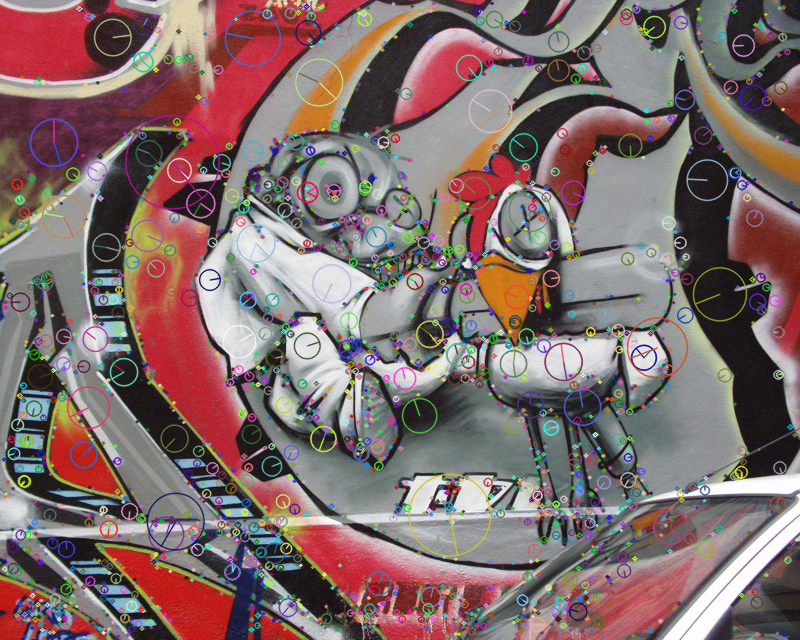
\includegraphics[width=0.65\textwidth]{images/RobotKp}
		\caption{Keypoints}
	\end{figure}
	\noindent
	La detecció es pot classificar en:\\
	\begin{itemize}
		\item{Detecció de vores}
		\item{Detecció de cantonades}
		\item{Detecció de regions\\}
	\end{itemize}
	Les principals tècniques d'obtenció de keypoints que s'han utilitzat són: SIFT, HARRIS i ORB.
	També s'han provat altres algorismes com FAST, SURF, STAR, MSER o SHI-TOMASI.

	\subsubsection{HARRIS}
	Harris és un detector que es basa en trobar cantonades. La idea bàsica és que mitjançant una finestra de NxM píxels, es recorre la imatge buscant els punts on hi ha canvis d'intensitat
	en diverses direccions.\\\\
	Segons els canvis d'intensitat de cada píxel, es poden classificar els punts en "flat", vores i cantonades.\\\\
	\begin{figure}[H]
		\centering
		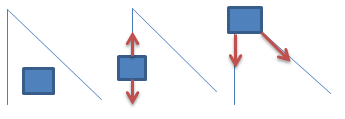
\includegraphics[width=0.7\textwidth]{images/harris}
		\caption{Flat, vora i cantonada}
	\end{figure}
	\noindent
	El problema principal de Harris és que no és invariant a l'escala. Punts considerats cantonades en una escala, podrien convertir-se en vores en una altra.
	Per això, existeixen algunes solucions com Harris-Laplace.\\\\
	En el nostre cas, s'ha optat per aplicar Harris en diverses escales, fent una piràmide de la imatge original.

	\subsubsection{SIFT}
	Localització multi-escala mitjançant una diferencia de gaussianes (DoG), que s'utilitza com a aproximació d'una laplaciana de gaussianes.\\\\
	Es troba l'histograma d'orientacions ponderat en l'escala calculada i es calcula l'orientació dominant.

	\subsubsection{ORB}
	El detector de ORB (Oriented FAST and Rotated BRIEF) utilitza el detector FAST amb modificacions per millorar el rendiment.\\\\
	FAST és un detector de cantonades enfocat a aconseguir els punts de manera molt ràpida, a canvi d'empitjorar una mica l'eficacia. S'agafa la intensitat d'un píxel i es compara amb el conjunt
	de N píxels veins que el rodejen.\\\\
	\begin{figure}[H]
		\centering
		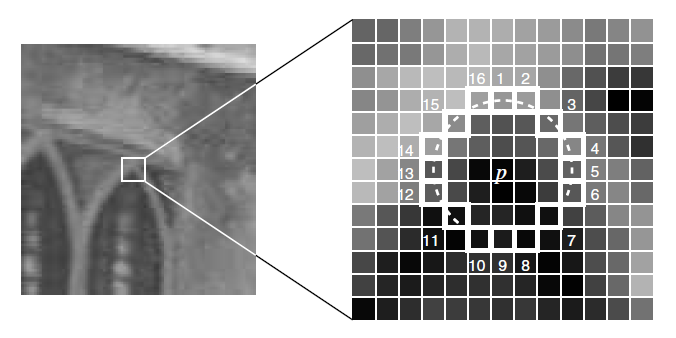
\includegraphics[width=0.55\textwidth]{images/fast}
		\caption{FAST}
	\end{figure}
	\noindent
	Suposant que N = 16 i definint un umbral t, si 12 píxels veins (\sfrac{3}{4} parts) són majors a I\textsubscript{p} + t o bé menors a I\textsubscript{p} - t, és considera que el punt és d'interès.
	El problema principal de FAST és que no té en compte l'orientació.\\\\
	ORB utilitza FAST aplicant les següents millores:\\
	\begin{itemize}
		\item{S'agafen els N millors punts despres d'aplicar la mesura de Harris.}
		\item{Es fa una piràmide per fer multi-escala.}
		\item{S'utilitzen els moments per calcular l'orientació.}
	\end{itemize}

\section{Extracció de característiques}

	L'extracció de característiques és el que ens permetrà comparar els punts obtinguts en les dues imatges.\\
	\begin{itemize}
		\item{Descriptors vectorials: SIFT, SURF}
		\item{Descriptors binaris: ORB, BRISK\\}
	\end{itemize}
	Principalment s'han utilitzat SIFT, ORB i BRISK, encara que també s'han provat d'altres com SURF, LATCH o DAISY.

	\subsubsection{SIFT}
	S'agafa l'histograma d'orientacions al voltant del punt, discretitzant en una finestra de 16x16.
	Es divideix en 16 particions de mida 4x4 i per cada partició es calcula un histograma d'orientacions, en 8 direccions.
	Finalment, es concatenen els histogrames per tal d'obtenir el vector de característiques de dimensió 128.
	\begin{figure}[H]
		\centering
		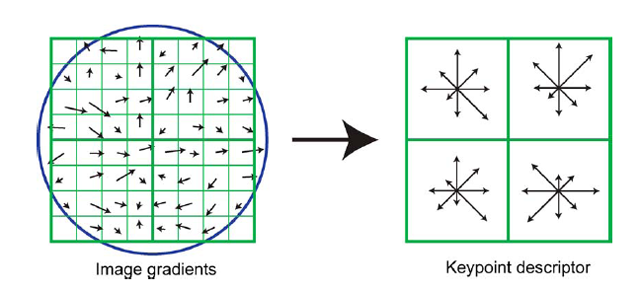
\includegraphics[width=0.65\textwidth]{images/sift-des}
		\caption{Descriptor SIFT}
	\end{figure}

	\subsubsection{ORB}
	El descriptor d'ORB és una modificació de BRIEF, un descriptor ràpid i senzill basat en strings binaris.\\\\
	Per cada keypoint s'agafen N punts veins i d'aquests s'agafen parells de forma mes o menys aleatoria. Per cada parell es compara la intensitat i es retorna un string binari de mida N amb '1' o '0' segons
	si la intensitat del primer punt és major a la del segon o no. Això ens permet comparar els descriptors amb una simple operació XOR.\\\\
	És un mètode molt ràpid pero no és invariable ni a la rotació ni a l'escala. Per això, ORB intenta solucionar el problema de la rotació girant els patrons en funció de l'angle de la característica.

	\subsubsection{BRISK}
	És un descriptor binari que utilitza un patró de cercles concentrics. S'agafen N punts del patró i per cada parell de punts es compara la intensitat del primer amb el segon. Si el valor del primer es
	major, es posa '1', sino '0'. D'aquesta manera s'obté una cadena d'N caràcters (binari) molt fàcil de comparar a l'hora de fer matching. Utilitizant el mateix patró i sequencia de parells, nomes caldrà
	comparar les cadenes binaries amb la suma del resultat d'una XOR.
	\begin{figure}[H]
		\centering
		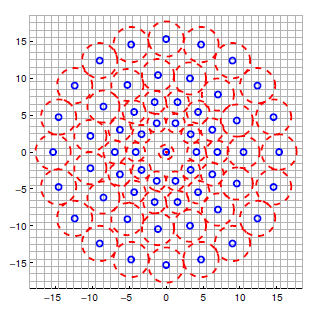
\includegraphics[width=0.5\textwidth]{images/brisk}
		\caption{Sampling pattern BRISK}
	\end{figure}


\newpage
\section{Matching de característiques}

	Un cop tenim els keypoints i les característiques dels punts, necessitarem obtenir coincidencies entre els punts de les dues imatges.\\\\
	Bàsicament podem obtenir els aparellaments de dues maneres:\\
	\begin{itemize}	
		\item{Força bruta: Consisteix en provar totes les combinacions possibles per cada punt.}
		\item{Aproximació\\}
	\end{itemize}
	Com que el temps d'execució no es una factor essencial, s'aplicarà el mètode de força bruta, una mica més lent. Pels descriptors binaris s'utilitzarà la distància de Hamming, mentre que pels vectorials
	s'utilitzarà l'euclidiana.\\

	\begin{figure}[H]
		\centering
		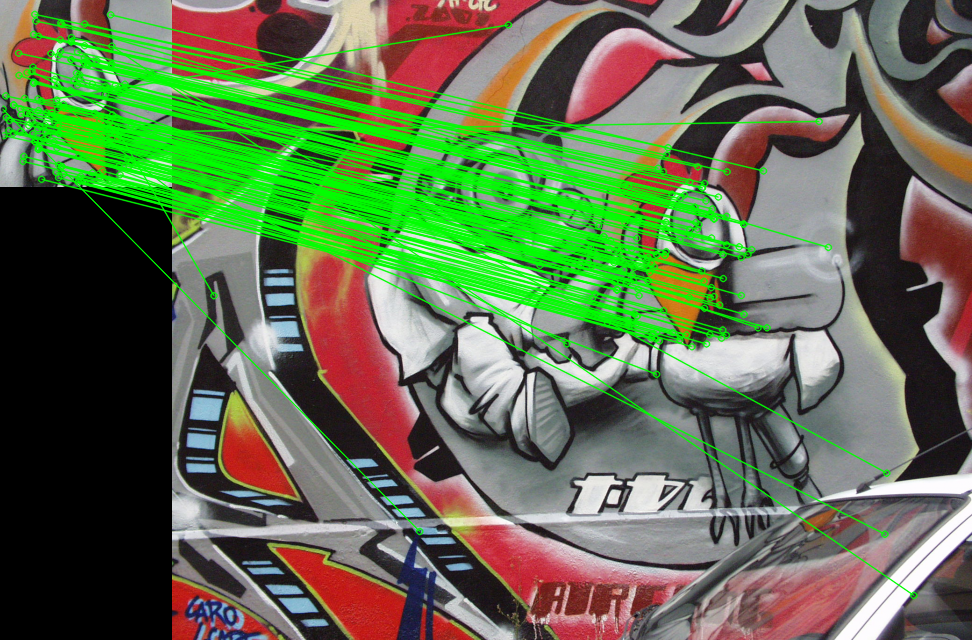
\includegraphics[width=0.7\textwidth]{images/matching}
		\caption{Matching}
	\end{figure}
\noindent
	En la imatge anterior podem veure determinats punts on el "match" és clarament erroni. Aquest error es pot minimitzar escollint punts més significatius, característiques més distinctives, aplicant el rati
	de Lowe o eliminant outliers.

\newpage
\section{Homografia}

	L'objectiu principal del programa es trobar una part d'una imatge en una altre imatge diferent i per fer això utilitzarem la homografia. Trobant la relació entre els píxels de les dues imatges podrem
	reprojectar el pla d'una imatge en l'altre i trobar el punt on volem dirigir el robot.\\
	\begin{figure}[H]
		\centering
		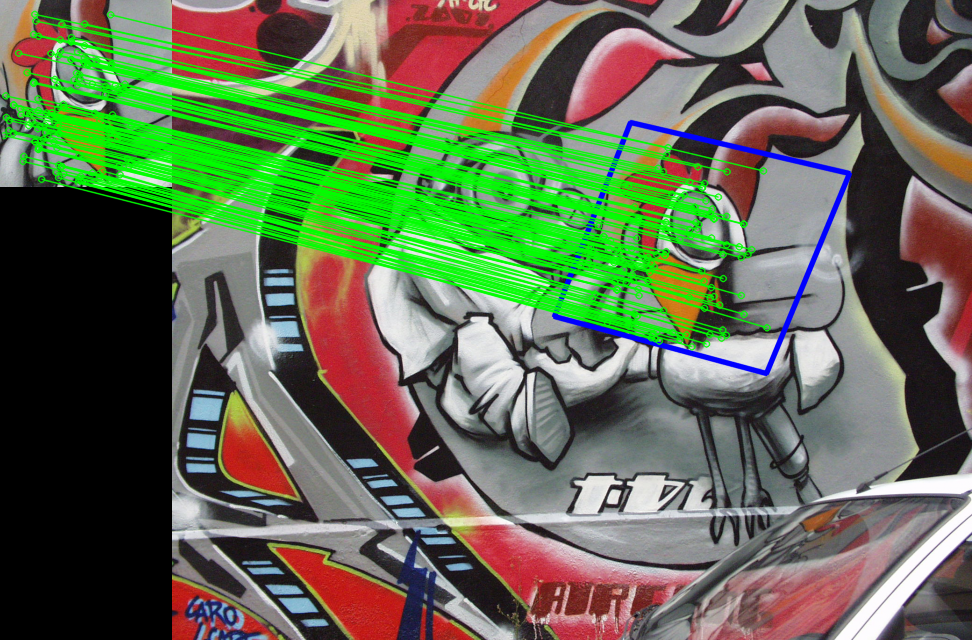
\includegraphics[width=0.7\textwidth]{images/homography}
		\caption{Homografia}
	\end{figure}
	\noindent
	A l'hora de buscar la homografia aplicarem RANSAC (Random Sample Consensus), un algorisme que ens permetrà eliminar outliers dels match trobats.\\
	\begin{figure}[H]
		\centering
		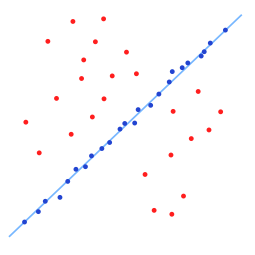
\includegraphics[width=0.45\textwidth]{images/ransac}
		\caption{Ransac}
	\end{figure}
